\section{The Standard Model}

Quantum Mechanics and the Theory of Special Relativity, along with the plethora of new particles discovered over the past century or so, has led to the formulation of the Standard Model of Particle Physics (SM)\cite{SM1}. It is a theory concerning the electromagnetic, weak\cite{EWT}, and strong nuclear interactions\cite{QCD}, as well as classifying all the subatomic particles known. It provides our best current understanding of the universe, what matter is made of and how it is held together. It rests on two basic ideas: all matter is made of particles, and these particles interact with each other by exchanging other particles associated with the fundamental forces. The basic components of matter are fermions and the force carriers are bosons and fermions have half-integer values of spin whereas bosons have integer values.

\begin{figure}[H]
\begin{center}
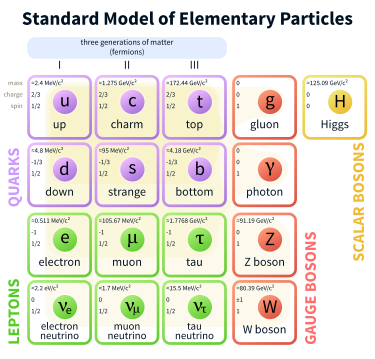
\includegraphics[width=0.5\textwidth]{SM.png}
\caption[Schematic representation of the Standard Model particles.]{Schematic representation of the Standard Model particles. Shown are the three generations of matter (formed by fermions), the gauge bosons and the Higgs boson.}
\label{SM} 
%\hspace{4em}
\end{center}
\end{figure}

Fermions come in two families as shown in \autoref{SM} - the leptons and quarks. The lepton family has six members, meanwhile the quark family contains six quarks. The up and down quarks are found inside protons and neutrons. The twelve fermions are the building blocks of matter and each one has a spin value of $\sfrac{1}{2}$. These particles interact with each other through fundamental forces. Each force comes with one or more force carriers. The nuclear force comes with the gluon and binds the quarks within the proton and neutrons. The photon is associated with the electromagnetic force and is responsible for mediating many of the forces humans encounter on a daily basis. The weak interaction is responsible for radioactivity and is mediated by the Z and W bosons. The gluons, photons and the Z and W bosons all have a spin of 1. The Standard Model is both remarkably simple and very powerful with nearly every measured quantity in particle physics laboratories over the past five decades falling right on the predicted value (within experimental error margins)\cite{SM2,SM3}. Until recently, the only missing piece of the SM was the Higgs boson\cite{Higgs1}. The Higgs boson is a particle corresponding to the Higgs field which, according to the SM, gives mass to all the fundamental particles. It was finally discovered at the LHC in 2012 \cite{Higgs,Higgs2}.

\section{Indications of Physics Beyond the Standard Model}

The Standard Model gives an incomplete picture of the makeup of the Universe as listed below:

\begin{enumerate}
	\item{The Standard Model does not include gravity and does not explain why gravity is so much weaker than the electromagnetic or nuclear forces\cite{hierarchy}. The weak force is $10^{24}$ times as strong as gravity. It is also incompatible with the most successful theory of gravity to date, general relativity\cite{GR1,GR2}.}
	\item{There is a wide spectrum of masses among the building blocks of matter\cite{massHierarchy}. Why? The electron is about 200 times lighter than the muon and 3,500 times lighter than the $\tau$-lepton, meanwhile the top quark is 75,000 times heavier than the up quark. Why is there such a wide spectrum of masses among the building blocks of matter?}
	\item{The SM introduces particle masses through a process known as spontaneous symmetry breaking\cite{SSB1,SSB2,SSB3} caused by the Higgs field. Within the standard model, the mass of the Higgs gets some very large quantum corrections due to the presence of virtual particles (mostly virtual top quarks). These corrections are much larger than the actual mass of the Higgs. This means that the bare mass parameter of the Higgs in the standard model must be fine-tuned in such a way that almost completely cancels the quantum corrections. This level of fine-tuning is deemed unnatural.}
	\item{It explains only about 5\% of matter  present in the universe. However, 26\% exists as dark matter\cite{WIMP} that behaves just like other matter (in terms of gravity) but which only interacts weakly (if at all) with the Standard Model fields. Yet, the Standard Model does not supply any fundamental particles that are good dark matter candidates. The rest (69\%) is dark energy\cite{DarkEnergy}, a constant energy density for the vacuum. Attempts to explain dark energy in terms of the standard model have failed.}
	\item{Neutrinos are predicted to be massless particles by the Standard Model\cite{NuMass}. However, neutrino oscillation experiments have shown that neutrinos do have mass\cite{NuMass1,NuMass2}. Mass terms for the neutrinos can be added to the standard model by hand, but these lead to new theoretical problems as these mass terms need to be extraordinarily small and it is doubtful if the neutrino masses would arise in the same way than the masses of other fundamental particles do in the Standard Model.}
	\item{The universe is made out of mostly matter but the standard model predicts that matter and antimatter should have been created in almost equal amounts if the initial conditions of the universe did not involve disproportionate matter relative to antimatter\cite{matterAntimatter}. But no mechanism, sufficient to explain matter--antimatter asymmetry, exists in the Standard Model.}
\end{enumerate}

Thus, as long as we observe various phenomena at low energy the Standard Model behaves properly, however, it lacks robustness at higher energy. To overcome its shortcomings several theories exists beyond the Standard Model that include various extensions of the standard model through supersymmetry, such as the Minimal Supersymmetric Standard Model (MSSM)\cite{MSSM,MSSM2} and Next-to-Minimal Supersymmetric Standard Model (NMSSM)\cite{NSSM1}, or entirely new ones like such as string theory\cite{StringTheory} and extra dimensions\cite{ExtraDimensions}. As these theories tend to reproduce the entirety of current phenomena, the question of which theory is the right one can only be determined by experiments. With the advent of even more powerful accelerators like the LHC, we are within reach of energy levels which existed only shortly after the Big Bang where the Standard Model has issues.

\section{Supersymmetric extension of the Standard Model}

The supersymmetry theories are based on a symmetry between fermions and bosons. It is similar to solving the `electron mass hierarchy problem' in quantum mechanics, where the number of particles is doubled: in addition to the electron, there is also a positron. The virtual electron--positron contributions solved the problem of electrons having a small mass by smearing out the electric charge. Supersymmetry is an analogous theory where once again the set of particles is doubled, and in doing so the loop contributions of one particle to the Higgs are cancelled by the loop contributions of its super-partner. It extends space-time symmetry since it relates matter particles to force particles. It relates particles with different spins but the same gauge charges.

\begin{figure}[H]
\begin{center}
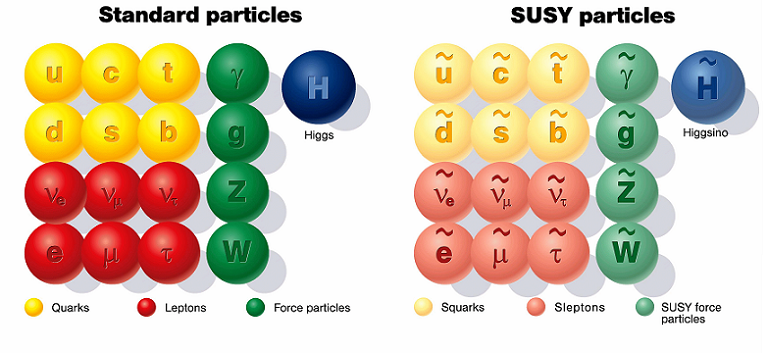
\includegraphics[width=0.9\textwidth]{SUSY.png} 
\caption[Schematic representation of the Standard Model particles with the added SUSY particles.]{Schematic representation of the Standard Model particles with the added SUSY particles.}
\label{SUSY} 
%\hspace{4em}
\end{center}
\end{figure}

The gluon (QCD) has a fermionic partner, the gluino. Similarly, the spin 1 gauge bosons W+, W0, W- and B$^0$ have their counterparts, called winos and binos, that, after electroweak symmetry breaking, mix to give the mass eigenstate Z$^0$ and $\gamma$, and the zino and photino respectively. For every lepton/quark there is a bosonic partner (i.e. a scalar slepton/squark). There are three families for each of the quark and lepton supermultiplets. The left-handed and right-handed pieces of the squarks and sleptons are two separate components, as in the corresponding SM sector. The Higgs doublet is extended by another doublet leading to other Higgs boson particles (Higgsinos).\\

Even though supersymmetry solves many problems in particle physics, it also poses new problems. If these new particles had the same mass as their counterparts in the standard model, we would have already observed them. Since none of these particles have been found yet, SUSY must be a broken symmetry. What makes superpartners heavier than ordinary particles? Why are superpartners so well hidden in rare phenomena? This arbitrary mass spectrum for the superpartners would have effects that are far too large in rare processes that change the flavor of particles. There must be some special reason why such effects are well hidden. How do we extract information on the mechanism of supersymmetry breaking? How does supersymmetry impact cosmology? Is the lightest supersymmetric partner what really composes Dark Matter? Different mechanisms have been suggested on how this symmetry is broken and have led to different phenomenological scenarios like the minimal supergravity model (mSUGRA)\cite{mSugra1,mSugra2}, the gauge-mediated supersymmetry breaking (GMSB)\cite{GMSB1,GMSB2,GMSB3} model or R-parity\cite{Rparity1,Rparity2}. A discussion of mSUGRA and GMSB is beyond the scope of this dissertation. R-parity is a new symmetry that has been added to the minimal supersymmetry scenario which prevents the violation of the leptonic and baryonic numbers. All SM fields have even R-parity, while SUSY particles have odd R-parity. The most obvious experimental constraint comes from the non-observation of proton decay \cite{pDecay1}, which would violate both baryonic and leptonic number conservation. Due to R-parity every interaction vertex in the theory involves an even number of sparticles, meaning that they must be pair-produced. The decay chains of the produced particles are characterized by the presence of one stable particle, generically called the Lightest Supersymmetric Particle (LSP), that may account for all the dark matter in the Universe. However, in other models, like the R-parity violating SUSY this may not apply. In other scenarios, those LSP can be regarded as vanishing mass and may not be enough to satisfy the dark matter in the Universe.

\subsection{Simplified Models Approach to Supersymmetry}

Simplified models \cite{SSM} are a new approach for characterizing LHC supersymmetry results. In a simplified model only a few new particles and a single decay topology are introduced, and hence these models are easy to constrain. Traditionally, testing a particle physics theory against experimental results requires calculating what the theory predicts in an experimental situation using a particle accelerator detector. This translates into computing: the masses of new particles, their decay widths, their branching ratios and production cross-sections. This information is subsequently used in Monte Carlo simulations of passage of proton-proton collisions products and their decays through the CMS detector. This is done under the hypothesis that the theory is true. The simulated data is  analyzed just like the actual experimental data resulting from proton-proton collisions. The theoretical and the experimental results can then be compared. Though conceptually uncomplicated it requires access to the experimental data, and the step of simulating the detector response requires intimate knowledge of the CMS detector by theorist community. It is also restrictive being model/theory dependent. The CMS collaboration, like ATLAS, does not share experimental details but only the final results via publications. The Simplified Model approach circumvents this issue by presenting results on very simple phenomenological models instead of a specific model, such as the constrained MSSM (cMSSM) \cite{cMSSM}. Each simplified models encompasses a specific phenomenological feature that is common to many different theories. A limited set of hypothetical particles and decay chains are introduced to produce a given topological signature. The amplitudes describing the production and decays of these particles are parametrized in terms of the particle masses and their branching ratios to daughter particles. This makes the analysis of simplified models less model dependent. The Simplified Models assume that a particular decay signature can be realized without specifying the exact mechanism, offering the possibility to overcome small branching ratios. Some Simplified Models with their corresponding production and decay modes are shown in the \autoref{topologyTable}. We have used T2tt, T1tttt, T1ttbb, T5tttt and T5ttcc models in analysis in this thesis. Some of these topologies are further discussed in more detail in \autoref{AnalysisChap}, since they correspond to some of the signals for SUSY in the treated analysis.

\begin{table}[H]
\begin{center}
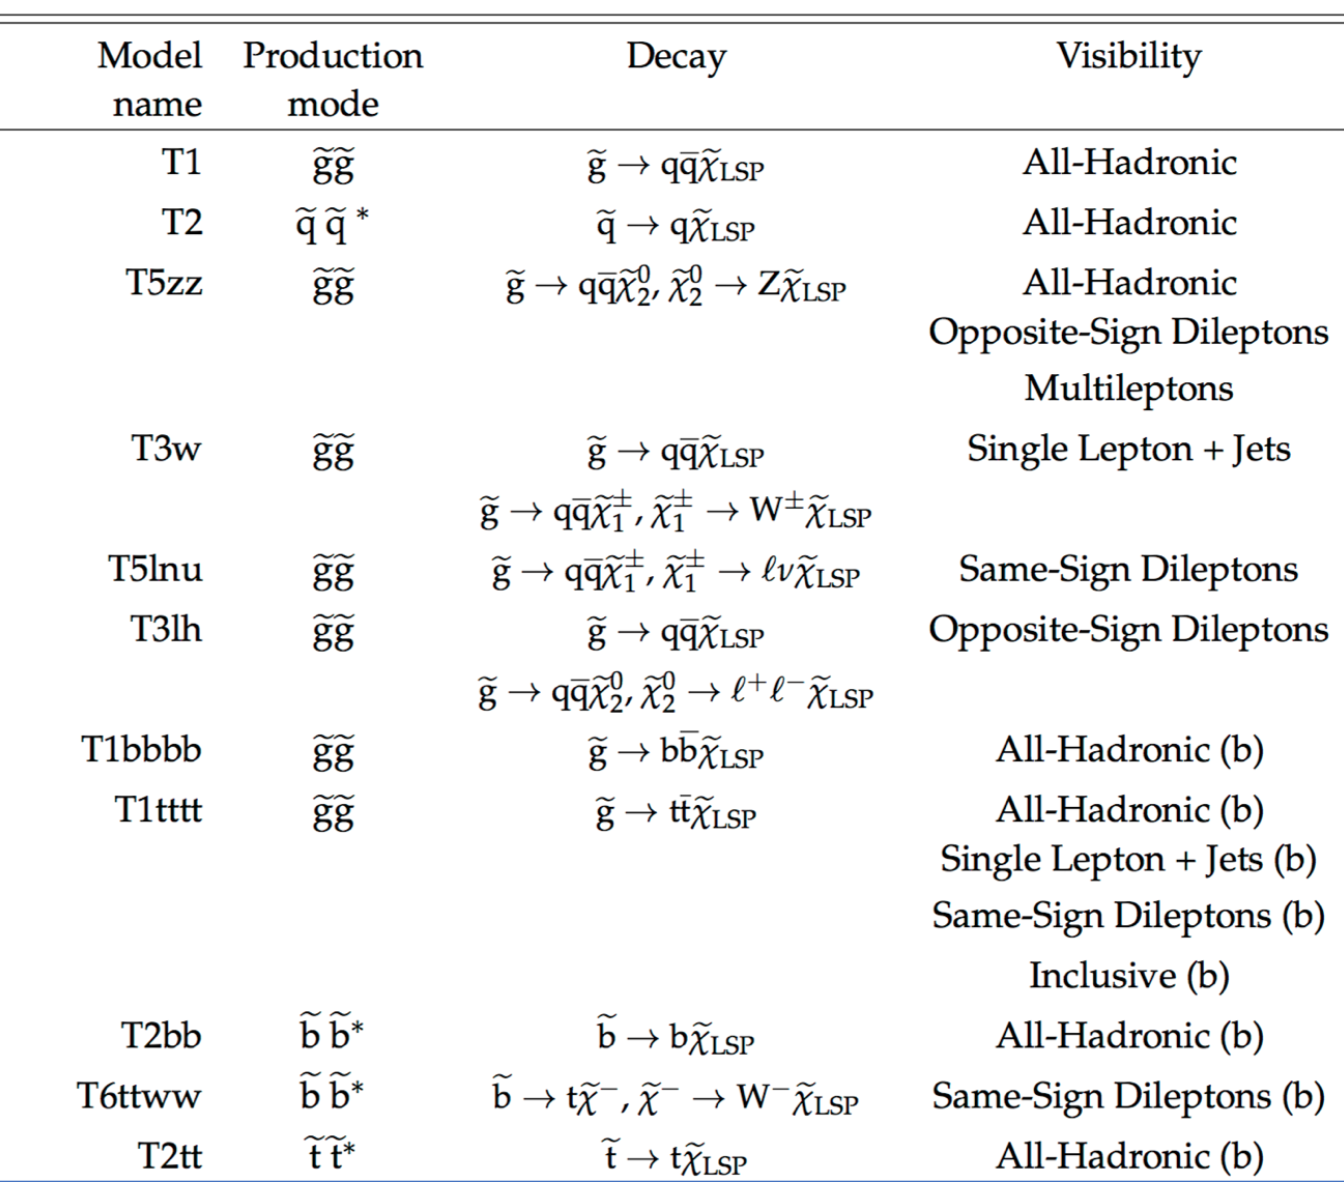
\includegraphics[width=0.9\textwidth]{topologyTable.png}
\caption{Some Simplified Models with their corresponding production and decay modes.}
\label{topologyTable}
\end{center}
\end{table}


